\documentclass[12pt,fleqn]{beamer}


\xdefinecolor{lavendar}{rgb}{0.8,0.6,1}
\xdefinecolor{olive}{cmyk}{0.64,0,0.95,0.4}
%\xdefinecolor{olive}{cmyk}{1,0,0,0}
\xdefinecolor{mag}{cmyk}{0.1,1,0,0.2}
\xdefinecolor{lblue}{rgb}{0,0,1.5}
\xdefinecolor{lred}{rgb}{1,0,0}
\xdefinecolor{mine}{cmyk}{1,0,0.2,0}
\xdefinecolor{bluel}{cmyk}{0.1,0,0.9,0.4}

\usepackage{amsmath,amssymb,dsfont,mathrsfs}
\usepackage{tikz,pgflibraryplotmarks}
\usepackage{multimedia}
\usepackage{wasysym}
\usepackage{rotating}
\usepackage{algorithm,algorithmic}
\usepackage{graphicx} % more modern
\usepackage{subfigure}
\usepackage{booktabs}

\usepackage{pgfplots}
\usepackage{verbatim}

\usepackage{setspace}
\newlength\iwidth
\newlength\iheight

\newcommand\makebeamertitle{\frame{\maketitle}}%
\graphicspath{{./images/}}
\setbeamertemplate{navigation symbols}{}
\addtobeamertemplate{navigation symbols}{}{%
    \usebeamerfont{footline}%
    \usebeamercolor[fg]{footline}%
	\insertshorttitle
    \;--
    \insertframenumber
}

\newcommand{\sectionstart}{
	\only<beamer>{
 	\begin{frame}% (fold)
 		\begin{centering}\Huge \insertsection \par\end{centering}
 	\end{frame}% frame the_application (end)
	}
 }


% make bibliography entries smaller
\usepackage{natbib}
\setbeamertemplate{bibliography item}{[\theenumiv]}
\renewcommand\bibfont{\scriptsize}
\setbeamertemplate{frametitle continuation}[from second]
\newcommand{\tcr}{\textcolor{red}}
\newcommand{\tcrd}{\textcolor{red}}
\newcommand{\tcb}{\textcolor{bluel}}
\newcommand{\tcm}{\textcolor{mag}}
\newcommand{\tcg}{\textcolor{olive}}

\newcommand{\R}{\mathbb{R}}
\newcommand{\C}{\mathbb{C}}

% bold lower-case for vectors
\newcommand{\bfa}{{\bf a}}
\newcommand{\bfb}{{\bf b}}
\newcommand{\bfc}{{\bf c}}
\newcommand{\bfs}{{\bf s}}
\newcommand{\bfm}{{\bf m}}
\newcommand{\bfd}{{\bf d}}
\newcommand{\bfe}{{\bf e}}
\newcommand{\bfu}{{\bf u}}
\newcommand{\bfy}{{\bf y}}
\newcommand{\bfx}{{\bf x}}
\newcommand{\bfh}{{\bf h}}
\newcommand{\bfw}{{\bf w}}
\newcommand{\bfv}{{\bf v}}
\newcommand{\bfr}{{\bf r}}
\newcommand{\bfz}{{\bf z}}
\newcommand{\bfp}{{\bf p}}


% bold upper-case for linear operators
\newcommand{\bfA}{{\bf A}}
\newcommand{\bfB}{{\bf B}}
\newcommand{\bfZ}{{\bf Z}}
\newcommand{\bfM}{{\bf M}}
\newcommand{\bfC}{{\bf C}}
\newcommand{\bfD}{{\bf D}}
\newcommand{\bfQ}{{\bf Q}}
\newcommand{\bfJ}{{\bf J}}
\newcommand{\bfG}{{\bf G}}
\newcommand{\bfI}{{\bf I}}
\newcommand{\bfP}{{\bf P}}
\newcommand{\bfK}{{\bf K}}
\newcommand{\bfY}{{\bf Y}}
\newcommand{\bfW}{{\bf W}}
\newcommand{\bfR}{{\bf R}}
\newcommand{\bfL}{{\bf L}}
\newcommand{\bfF}{{\bf F}}
\newcommand{\bfT}{{\bf T}}
\newcommand{\bfS}{{\bf S}}
\newcommand{\bfX}{{\bf X}}
\newcommand{\bfU}{{\bf U}}
\newcommand{\bfV}{{\bf V}}
\newcommand{\bfH}{{\bf H}}


\newcommand{\calF}{\mathcal{F}}



\newcommand{\hf}{{\frac 12}}
\newcommand{\bftheta}{{\boldsymbol \theta}}
\newcommand{\bfxi}{{\boldsymbol \xi}}

\newcommand{\bfLambda}{{\boldsymbol \Lambda}}
\newcommand{\bfSigma}{{\boldsymbol \Sigma}}
\newcommand{\bfepsilon}{{\boldsymbol \epsilon}}

\newcommand{\E}{\vec E}
\newcommand{\B}{\vec B}

\newcommand{\vu}{  {\vec {\bf u}}}

\newcommand{\grad}{  {\vec {\bf \nabla}}}

\newcommand{\lfrownie}{\textcolor{red}{\large{\frownie}}}
\newcommand{\lsmiley}{\textcolor{green}{\large{\smiley}}}

\newcommand{\curl}{\ensuremath{\nabla\times\,}}
\renewcommand{\div}{\nabla\cdot\,}
\newcommand{\divh}{\nabla_h\cdot\,}
\renewcommand{\grad}{\ensuremath{\nabla}}

\DeclareMathOperator*{\argmin}{arg\,min}

\title[Intro]{Introduction}
\subtitle{Numerical Methods for Deep Learning}
\date{}

\begin{document}


\makebeamertitle
\section{Course Overview} 
\label{sec:course_overview}
\begin{frame}
\frametitle{Course Overview}
\begin{itemize}
\item Module 1: Linear Models
\begin{enumerate}
	\setcounter{enumi}{1}	
\item Linear Models and Least-Squares
\item Iterative Methods for Least-Squares
\item Linear Models for Classification
\item Newton's Method for Classification
\item Regularization for Image Classification
\end{enumerate}
\end{itemize}

\end{frame}
\begin{frame}
\frametitle{Course Overview}

\begin{itemize}
\item Module 2: Neural Networks
\begin{enumerate}
	\setcounter{enumi}{6}
\item Introduction to Nonlinear Models
\item Single Layer Neural Networks
\item Training Algorithms for Single Layer Neural Networks
\item Introduction to Deep Neural Networks
\item Differentiating Deep Neural Networks
\item Stochastic Gradient Descent and Variants
\end{enumerate}
\item Module 3: Parametric Models/Convolution Neural Networks
\begin{enumerate}
	\setcounter{enumi}{12}
	\item Introduction to Parametric Models
	\item Application of CNN: Image Segmentation
	\item CNN and their relation to PDEs
\end{enumerate}
\end{itemize}
\end{frame}




% section course_overview (end)


\section{Introduction to (Deep) Neural Networks} % (fold)
\label{sec:introduction_to_deep_neural_networks}

\begin{frame}\frametitle{{Neural Networks: History}}

\begin{itemize}
	\item Neural Networks with a particular (deep) architecture
    \item Exist for a long time (70's and even earlier)~\cite{Rosenblatt1958,Rumelhart1986,LeCun1990}
    \item Recent revolution - computational power and lots of data~\cite{bengio2009learning,RainaEtAl2009,lecun2015deep}
    \item Can perform very well for large amounts of data
    \item Applications
    \begin{itemize}
    \item Image recognition~~\cite{hinton2012deep,KrizhevskySutskeverHinton2012,lecun2015deep}, segmentation, natural language processing~\cite{BordesEtAl2014,CollobertEtAl2011,  JeanEtAl2014}
    \end{itemize}


    \pause

\item A few recent news articles:

 \begin{itemize}
    \item
{Apple Is Bringing the AI Revolution to Your iPhone, WIRED 2016}
\item
{Why Deep Learning Is Suddenly Changing Your Life,  FORTUNE 2016}
\item Data Scientist: Sexiest Job of the 21st Century, Harvard Business Rev ’17
\end{itemize}

\end{itemize}
\end{frame}

\begin{frame}\frametitle{NN - A Quick Overview}

Neural Networks is a data interpolator/classifier when the underlying model
is unknown.

\bigskip

A generic way to write it is
$$ \bfc = f(\bfy,\bftheta). $$


\begin{itemize}
\item The function $f$ is the computational model.
\item $\bfy\in\R^{n_f}$ is the input data (e.g., an image)
\item $\bfc\in\R^{n_c}$ is the output (e.g. class the image)
\item $\bftheta\in\R^{n_p}$ are parameters of the model $f$
\end{itemize}

In learning we have examples $\{(\bfy_j,\bfc_j) \ : \ j=1,\ldots,n\}$ and the goal
is to estimate or ``learn'' the parameters $\bftheta$

\end{frame}


\begin{frame}\frametitle{Learning From Data: The Core of Science}


Given inputs and outputs, how to choose $f$?

\bigskip

Option 1 (Fundamental(?) understanding): For example, Newton's formula
$$ x(t) = \hf g t^2, $$
with unknown parameter $g$. 

\pause

To estimate $g$ observe falling object
\begin{center}
\begin{tabular}{cc}
t   &  x \\ \hline
0  &  0  \\
1  & 4.9  \\
2  & 20.1 \\
3  & 44.1 \\
\end{tabular}
\end{center}
What is the optimal value for $g$?




\end{frame}


\begin{frame}\frametitle{Learning From Data: The Core of Science}



Given inputs and outputs, how to choose $f$?

\bigskip

Option 2 (Phenomenological models): For example, Archie's law - what is the electrical resistivity of a rock
 and how it relates to its porosity, $\phi$ and saturation, $S_w$?
$$ \rho(\phi,S_w) = a \phi^{n/2} S_w^p $$
$a,n,p$ unknown parameters


\bigskip

Obtaining parameters from observed data and lab experiments on rocks


\end{frame}


\begin{frame}\frametitle{Phenomenological vs. Fundamental}

\textbf{Fundamental laws} come from understanding(?) the underlying process.
They are {\bf assumed invariant} and can therefore be predictive(?).

\bigskip

\textbf{Phenomenological models} are data driven. They ``work'' on some given data.
Hard to know what are the limitations.

\bigskip

{\bf But ...}
\begin{itemize}
\item models based on understanding can do poorly - weather, economics ...
\item models based on data can sometimes do better
\item how do we quantify understanding?
\end{itemize}

\end{frame}


\begin{frame}\frametitle{Generalization}

Suppose that we have examples $\{\bfy_j,\bfc_j\},\ \ j=1,\ldots,n$,
a model $f(\bfy,\bftheta)$ and some optimal parameter $\bftheta^*$.

Let $\{(\bfy^t_j,\bfc^t_j) \ : \  j=1,\ldots,s\}$ be some test set, that was not used
to compute $\bftheta^*$.

\pause

Loosely speaking, if
$$ \|f(\bfy^t_j,\bftheta^*) - \bfc_j^t\|_p \text{ is small}$$
then the model is predictive - it generalizes well



\pause
\bigskip


For phenomenological models, there is no reason why the model
should generalize, but in practice it often does.


\end{frame}

\begin{frame}\frametitle{Generalization}


Why would a model generalize poorly?
$$ 1 \ll \|f(\bfy^t_j,\bftheta^*) - \bfc_j^t\|_p $$

\bigskip
\pause

Two common reasons:
\begin{enumerate}
\item Our ``optimal'' $\bftheta^*$ was optimal for the training but is less so for other data
\item The chosen computational model $f$ is poor (e.g. linear model for a nonlinear function).
\end{enumerate}


\end{frame} 
\begin{frame}\frametitle{Example: Classification of Hand-written Digits }

\begin{itemize}
\item
Let $\bfy_j \in \R^{n_f}$ and let $\bfc_j\in \R^{n_c}$.
\item
The vector $\bfc$ is the probability of $\bfy$ belonging to a certain class. Clearly, $0\le \bfc_j \le 1$ and $\sum_{j=1}^{n_c} \bfc_j = 1$.
\end{itemize}

\vfill

Examples (MNIST):
\begin{center}
	\begin{tabular}{cc}
		$\bfy_1$ & $\bfy_2$\\
	\includegraphics[width=30mm]{maybe4} &
	\includegraphics[width=30mm]{maybe7} \\
	$\bfc_1 = [0, 0, 0, 0, 1, 0, 0, 0, 0, 0]^\top$ &
	$\bfc_2 = [0, 0.3, 0, 0, 0, 0, 0, 0.7, 0, 0]^\top$
	\end{tabular}
	
\end{center}


\end{frame} 
\begin{frame}\frametitle{Example: Classification of Natural Images}

Image classification of natural images
\bigskip

Examples (CIFAR-10):
\begin{center}
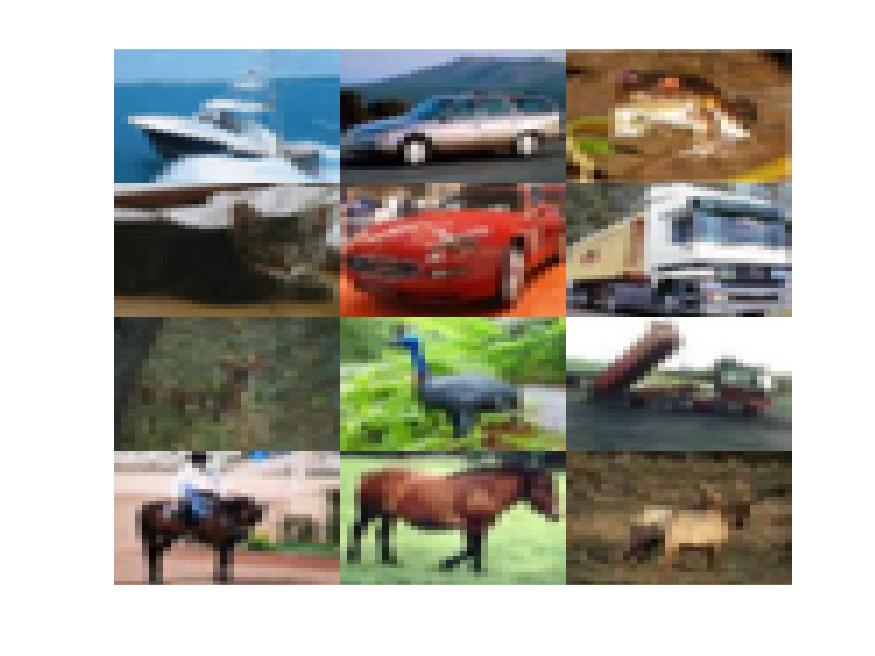
\includegraphics[width=9.5cm]{cifar10Sample.jpg} 
\end{center}

\end{frame}
 
\begin{frame}\frametitle{Example:  Semantic Segmentation}

\begin{itemize}
	\item
	let $\bfy_j \in \R^n$ be an RGB or grey valued image.
	\item let the pixels in $\bfc_j\in \{1,2,3,\ldots \}^k$ denote the labels.
\end{itemize}

\begin{center}
	\begin{tabular}{cc}
		$\bfy$, input image & $\bfc$, segmentation (labeled image)\\
	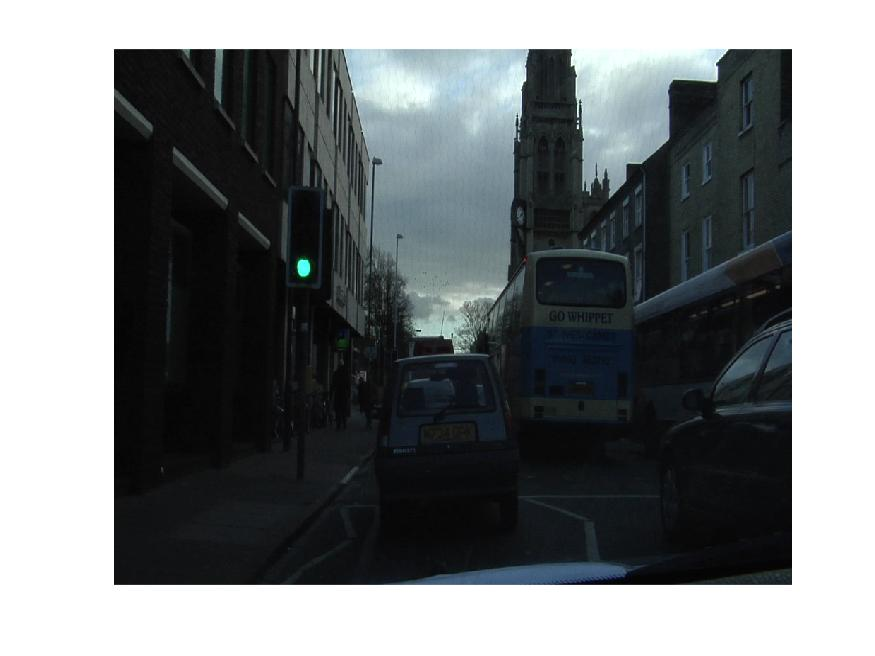
\includegraphics[width=5.5cm]{camvidPic.jpg} &
	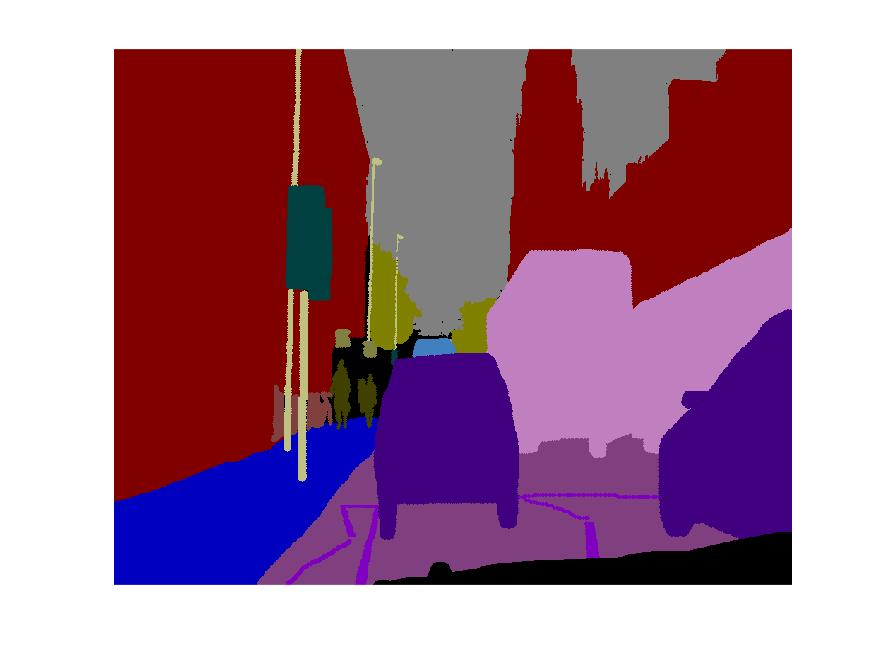
\includegraphics[width=5.5cm]{camvidClass.jpg} 
	\end{tabular}

	Goal: Find map $\bfc  = f(\bfy,\bftheta)$ 

\end{center}


\end{frame}

\begin{frame}\frametitle{Example 3: Semantic Segmentation}

Problem: Given image $\bfy$ and label $\bfc$ find a map $f(\cdot,\bftheta)$ such that $\bfc  \approx f(\bfy,\bftheta)$ 

\bigskip
\pause

First step: Reduce the dimensionality of problem.
\begin{itemize}
\item extract features from the image
\item classify in the feature space
\end{itemize}

Reduce the problem of learning from the image to feature
detection and classification

\pause
\bigskip

Possible features: Color, neighbors, edges ...

\bigskip


\end{frame}


\begin{frame}\frametitle{Example 3 - Semantic Segmentation}


Simpler setup
\begin{itemize}
\item data, $\bfy$ is the RGB value of the pixel (and its neighbors?)  
\item $\bfc$ is a labeled pixel
\item The map $\bfc  = f(\bfy,\bftheta)$ 
\end{itemize}

\begin{tabular}{cc}
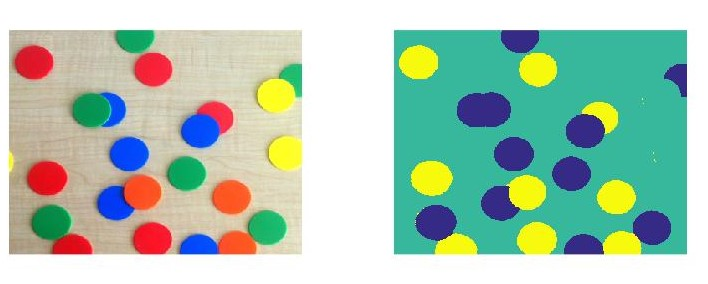
\includegraphics[width=5.5cm]{circles.jpg} &
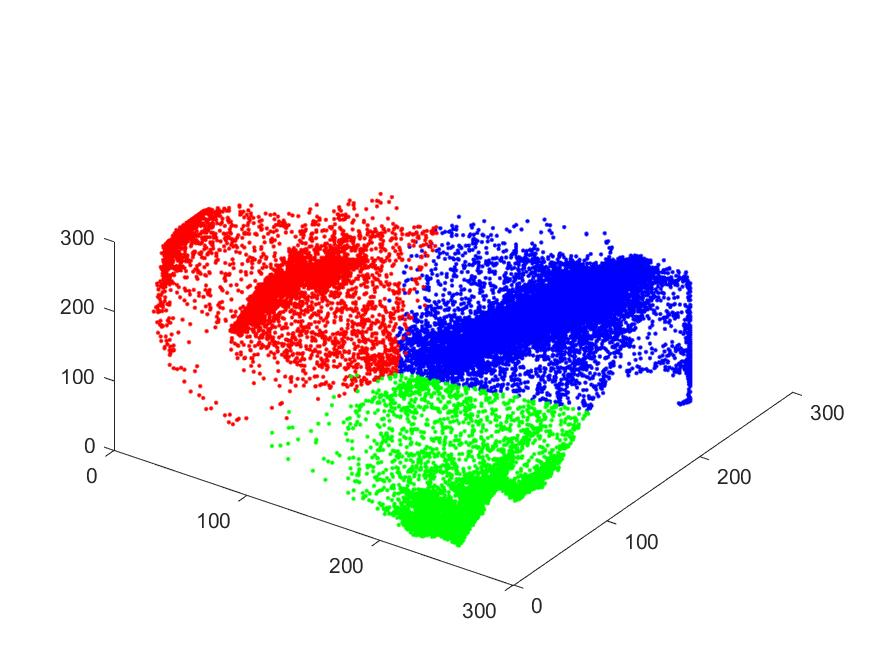
\includegraphics[width=4.5cm]{circlesFeatSpace.jpg} \\
input image and segmentation & 3D representation of RGB values \\
\end{tabular}

\end{frame}

\begin{frame}\frametitle{Coding: Download Data and Setup MATLAB}

The following data sets will be used throughout the course (and homework projects).

\bigskip

The following are ordered from small and easy to large and challenging:
\begin{itemize}
	\item MNIST
	\item CIFAR-10
	\item CamVid: download from Mathworks web page. 
\end{itemize}

\end{frame}

\begin{frame}[allowframebreaks]
	\frametitle{References}
 \bibliographystyle{abbrv}
\bibliography{NumDNN}

\end{frame}

\end{document}






